%%%%%%%%%%%%%%%%%%%%%%%%%%%%%%%%%%%%%%%%%%%%%%%%%%%%%%%%%%%%%%%%%%%%%%%%%%%%%%%%%%
% The Ascon state
%
% public domain (CC0 1.0 https://creativecommons.org/publicdomain/zero/1.0/)
%%%%%%%%%%%%%%%%%%%%%%%%%%%%%%%%%%%%%%%%%%%%%%%%%%%%%%%%%%%%%%%%%%%%%%%%%%%%%%%%%%



\newif\ifsans
\newif\iftext
\newif\ifcolor

%%% CONFIGURATION %%%%%%%%%%%%%%%%%%%%%%%%%%%%%%%%%%%%%%%%%%%%%%%%%%%%%%%%%%%%%%%%
%\sanstrue   % for sans-serif fonts (slides, web)
\sansfalse % for serif fonts (article)

\texttrue   % include phase description
%\textfalse % no phase description

\colortrue   % use color for highlights
%\colorfalse % no color

%\horizontaltrue % highlight horizontal word
%\verticaltrue % highlight vertical slice
%\constanttrue % highlight vertical slice
%%%%%%%%%%%%%%%%%%%%%%%%%%%%%%%%%%%%%%%%%%%%%%%%%%%%%%%%%%%%%%%%%%%%%%%%%%%%%%%%%%

\usetikzlibrary{shadows}
\ifcolor
  \definecolor{webred}{HTML}{D35400}
\else
  \definecolor{webred}{HTML}{444444}
\fi

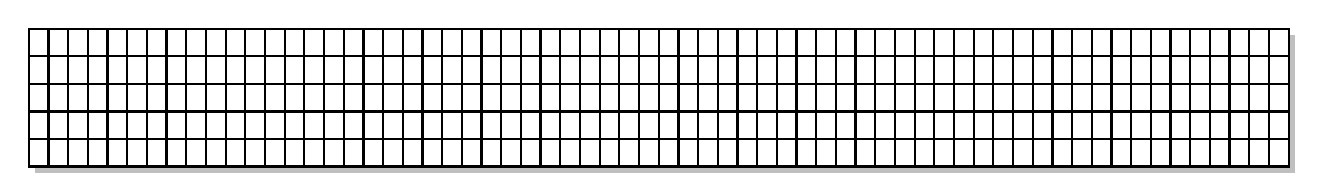
\begin{tikzpicture}[thick, scale=0.5]
  \draw[fill=white, drop shadow] (0,0) rectangle (32,3.5);
  \draw (0,.7) -- (32,.7)
                (0,1.4) -- (32,1.4)
                (0,2.1) -- (32,2.1)
                (0,2.8) -- (32,2.8);
                
  \foreach \x in {1,...,63}
  \draw (0.5*\x, 0) -- (.5*\x, 3.5);
  
  \iftext
    \draw (33,.35) node {$X_4$}
         ++(0,.7) node {$X_3$}
         ++(0,.7) node {$X_2$}
         ++(0,.7) node {$X_1$}
         ++(0,.7) node {$X_0$};
  \fi

\end{tikzpicture}